\documentclass[letterpaper,10pt]{extarticle}
\usepackage[utf8]{inputenc}
\usepackage[T1]{fontenc}
\usepackage{graphicx}
\usepackage[x11names]{xcolor}
\usepackage{tikz}
% \usetikzlibrary{circuits.ee.IEC}
\usepackage[american,cuteinductors,smartlabels]{circuitikz}

\usetikzlibrary{calc}
\ctikzset{bipoles/thickness=1}
\ctikzset{bipoles/length=0.8cm}
\ctikzset{bipoles/diode/height=.375}
\ctikzset{bipoles/diode/width=.3}
\ctikzset{tripoles/thyristor/height=.8}
\ctikzset{tripoles/thyristor/width=1}
\ctikzset{bipoles/vsourceam/height/.initial=.7}
\ctikzset{bipoles/vsourceam/width/.initial=.7}
\tikzstyle{every node}=[font=\small]
\tikzstyle{every path}=[line width=0.8pt,line cap=round,line join=round]

\usepackage[os=win]{menukeys}

\usepackage{amsmath,amssymb,textcomp}
\everymath{\displaystyle}

\usepackage{physics}

\usepackage{siunitx}
\usepackage{standalone}
\usepackage{times}
\renewcommand\familydefault{\sfdefault}
\usepackage{tgheros}
\usepackage{droidmono}

\usepackage{enumitem}
\usepackage[explicit]{titlesec}

\usepackage{multicol}
\setlength{\columnseprule}{0pt}
\setlength{\columnsep}{15.0pt}

\usepackage{geometry}
\geometry{left=10mm,right=10mm,top=10mm,bottom=15mm,showframe=false}

% custom title
\makeatletter
\renewcommand*{\maketitle}{%
\noindent
\begin{minipage}{0.82\textwidth}

\begin{tikzpicture}
\node[rectangle,rounded corners=6pt,inner sep=6pt,fill=SteelBlue1,text width=.95\textwidth] {\color{black}\huge \@title};
\end{tikzpicture}
\end{minipage}
\hfill
\begin{minipage}{0.17\textwidth}
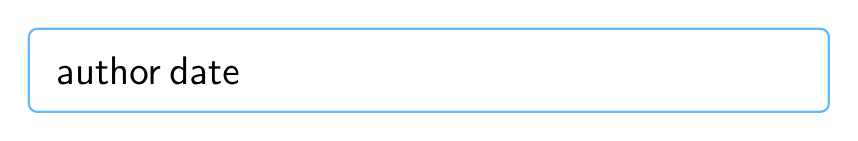
\begin{tikzpicture}
\node[rectangle,rounded corners=3pt,inner sep=10pt,draw=SteelBlue1,text width= 0.78\textwidth] {\raggedleft \Large \@author\ \@date};
\end{tikzpicture}
\end{minipage}
%\bigskip%\bigskip
}%
\makeatother

% custom section
\newcommand*\sectionlabel{}
\titleformat{\section}
  {\gdef\sectionlabel{}
   \normalfont\sffamily\Large\bfseries\scshape}
  {\gdef\sectionlabel{\thesection\ }}{0pt}
  {
\noindent
\begin{tikzpicture}
\node[rectangle,rounded corners=3pt,inner sep=4pt,fill=DodgerBlue4,text width= 0.95\columnwidth] {\color{white}\sectionlabel#1};
\end{tikzpicture}
  }
\titlespacing*{\section}{0pt}{.5pt}{0.5pt}

% custom subsection
\newcommand*\subsectionlabel{}
\titleformat{\subsection}{\normalfont\sffamily\bfseries\scshape}{\subsectionlabel}{0pt}{
\noindent
\begin{tikzpicture}
\node[rectangle,rounded corners=4pt,inner sep=3pt,fill=DodgerBlue3,text width= 0.95\columnwidth] {\color{white}\subsectionlabel#1};
\end{tikzpicture}
}
\titlespacing*{\subsection}{0pt}{.5pt}{.5pt}

% custom subsubsection
\newcommand*\subsubsectionlabel{}
\titleformat{\subsubsection}{\normalfont\sffamily\small\bfseries\scshape}{\subsubsectionlabel}{0pt}{
\noindent
\begin{tikzpicture}
\node[rectangle,rounded corners=3pt,inner sep=3pt,fill=blue!50!yellow,text width= 0.95\columnwidth] {\color{white}\subsubsectionlabel#1};
\end{tikzpicture}
}
\titlespacing*{\subsubsection}{0pt}{.5pt}{.5pt}


\title{GPA325 : Introduction à l'électronique}
\author{INTRA}
\date{A2019}

%\linespread{1.3}

\begin{document}
\maketitle

\begin{multicols*}{2}

\setlength{\belowdisplayskip}{2.5pt}
\setlength{\belowdisplayshortskip}{2.5pt}
\setlength{\abovedisplayskip}{2.5pt}
\setlength{\abovedisplayshortskip}{2.5pt}


\section{Notion de base}
\vspace{-1.75\baselineskip}
\begin{tabular}{ll}
Puissance électrique & \(P = VI = R I^2 = V^2/R\)\\
Loi d'Ohm & \(V = RI \Leftrightarrow R=V/I \)\\
Résistances en série & \(R_{\mathit{eq}}=R_1 + \dots + R_N\)\\
Résistances en parallèle & \(R_{\mathit{eq}}=\qty(\frac{1}{R_1}+\dots +\frac{1}{R_N})^{-1}\)
\end{tabular}

\subsection{Kirchhoff}
\begin{center}
\begin{tabular}{c|c}
    Loi des noeuds & Loi des mailles \\
    % $\Sigma I = 0$ & $\Sigma \Delta V =0$
    $\sum I = 0$ & $\sum \Delta V =0$
\end{tabular}
\end{center}

% \subsubsection{Étapes de résolution d'un circuit}
% \begin{enumerate}[nosep]
%     \item Assigner un courant dans chaque branche : Direction arbitraire, si le courant est négatif, alors le courant circule en sens contraire.
%     \item Écrire les équations de tous les noeuds sauf un. $(n-1)$
%     \item Écrire les équations de diverses mailles jusqu'à l'obtention de $X$ équations pour $X$ inconnues; chaque branche doit être parcourue aux moins une fois.
% \end{enumerate}
% \subsubsection{Sens du courant}


%\section{Techniques d’analyse de circuits}
% \vspace{-.5\baselineskip}
% \subsection{Transformation de source}
% \vspace{-1\baselineskip}
% Seulement possible s'il n'y a pas de source dépendante dans le circuit.
% \begin{multicols*}{2} 
% \centering
%  trim={<left> <lower> <right> <upper>}
% \includegraphics[trim={1.75in 8.375in 1.75in 1in}, clip=true,page=2,height=.85in]{fig/equiv.pdf}

% \begin{equation*}
%     I_s = \frac{V_s}{R}
% \end{equation*}
% \end{multicols*}
% \vspace{-1\baselineskip}

% % \vspace{-1\baselineskip}
% \subsubsection{Cas particulier}
% \begin{itemize}[nosep]
%     \item Résistance en $//$ avec $V_s$ peut être ignorée.
%     \item Résistance en série avec $i_s$ peut être ignorée.
% \end{itemize}


% \subsection{Équivalents Thévenin et Norton}
% \begin{equation*}
%     R_{Th}=\frac{V_{Th}}{I_{cc}}
% \end{equation*}
% Cas particulier, si le circuit n'a pas de source dépendante. 
% \begin{itemize}[nosep]
%     \item Source de tension $=$ court-circuit
%     \item Source de courant $=$ circuit ouvert
% \end{itemize}
% \subsubsection{Étapes de résolution}
% \begin{enumerate}[nosep]
%     \item Calculer la tension de Thévenin $V_{Th}$
%     \item Calculer le courant de court-circuit $I_{cc}$
%     \item Calculer la résistance de Thévenin $R_{Th}$
%     \item Re-dessiner le circuit équivalent Thévenin
% \end{enumerate}

% \subsubsection{Équivalent Norton}
% On obtient l'équivalent Norton en faisant une transformation de source de l'équivalent Thévenin.


% \subsection{Transfert maximal de puissance}
% La puissance consommée par la charge $R_L$ est: 
% %\vspace{-.5\baselineskip}
% \begin{equation*}
%     P = VI = R_L I^2 = R_L \qty(\frac{V_{Th}}{R_{Th}+R_L})^2
% \end{equation*}
% Résistance $R_L$ pour obtenir un transfert de puissance maximal
% %\vspace{-1\baselineskip}
% \begin{equation*}
%     R_L = R_{Th}
% \end{equation*}
% La puissance transférée à la charge:
% %\vspace{-.375\baselineskip}
% \begin{equation*}
%     P_{max} = \frac{V^2_{Th}}{4R_L}
% \end{equation*}
% %\vspace{-1\baselineskip}
\section{Redresseurs}
\renewcommand{\arraystretch}{1.25}
\begin{tabular}{ll}
    Tension pointe à l'entrée & \( V_{2p}= \sqrt{2}*V_{RMS} * N_2/N_1\)\\
    Si la diode est idéale & \(V_{\mathrm{seuil}}=0\)
\end{tabular}

\subsection{sans filtrage}
\subsubsection{Simple alternance}
\begin{tabular}{ll}
    Paramètre & Diode réelle \\\hline
    Tension pointe de la charge & \(V_{Lp}=V_{2p}-V_{\mathrm{seuil}}\)\\
    Tension moyenne de la charge & \(V_{L\mathrm{moy}}=V_{2p}-V_{\mathrm{seuil}}/\pi \)\\
    Courant moyen dans la charge & \(I_{L\mathrm{moy}}=V_{2p}-V_{\mathrm{seuil}}/\pi R_{L} \)\\
    Courant moyen dans la diode &  \(I_{D\mathrm{moy}}=V_{2p}-V_{\mathrm{seuil}}/\pi R_{L} \)\\
    Tension inverse de crête & \(TIC=V_{2p}\)
\end{tabular}

\subsubsection{Double alternance}
\renewcommand{\arraystretch}{2}
\begin{tabular}{ll}
    Paramètre & Diode réelle \\\hline
    Tension pointe de la charge & \(V_{Lp}=\frac{V_{2p}}{2}-V_{\mathrm{seuil}}\)\\
    Tension Moyenne de la charge & \(V_{L\mathrm{moy}}=\frac{V_{2p}-2V_{\mathrm{seuil}}}{\pi}\)\\
    Courant moyen dans la charge & \(I_{L\mathrm{moy}}=\frac{V_{2p}-2V_{\mathrm{seuil}}}{\pi R_L}\)\\
    Courant moyen dans les diodes &  \(I_{D\mathrm{moy}}=\frac{V_{2p}-2V_{\mathrm{seuil}}}{2\pi R_L}\)\\
    Tension inverse de crête & \(TIC_{D1} = TIC_{D2}=V_{2p}\)
\end{tabular}

\subsubsection{en pont}
\begin{tabular}{ll}
    Paramètre & Diode réelle \\\hline
    Tension pointe de la charge & \(V_{Lp}=V_{2p}-2V_{\mathrm{seuil}}\)\\
    Tension moyenne de la charge & \(V_{L\mathrm{moy}}=\frac{2(V_{2p}-2V_{\mathrm{seuil}})}{\pi}\)\\
    Courant moyen dans la charge & \(I_{L\mathrm{moy}}=\frac{2(V_{2p}-2V_{\mathrm{seuil}})}{\pi R_L}\)\\
    Courant moyen dans les diodes &  \(I_{D\mathrm{moy}}=\frac{V_{2p}-2V_{\mathrm{seuil}}}{\pi R_L}\)\\
    Tension inverse de crête & \(TIC_{Di}=V_{2p}\)
\end{tabular}

\subsection{avec filtrage}
\renewcommand{\arraystretch}{1}
\subsubsection{Simple alternance $f=f_{\mathrm{in}}$}
\begin{center}
    \includestandalone[scale=1.25]{fig/redresseur_avec_filtrage}
\end{center}
\begin{tabular}{ll}
    Paramètre & Diode réelle \\\hline
    Tension pointe de la charge & \(V_{Lp}=V_{2p}-V_{\mathrm{seuil}}\)\\
    Tension moyenne de la charge & \(V_{L\mathrm{moy}}=V_{Lp}-(V_{R}/2)\)\\
    Ondulation de la tension & \(V_{R}=V_{Lp}/(R_L f C)\)\\
    Courant moyen dans la charge & \(I_{L\mathrm{moy}}=V_{L\mathrm{moy}}/R_{L} \)\\
    Courant moyen dans la diode &  \(I_{D\mathrm{moy}}=I_{L\mathrm{moy}}\)\\
    Courant maximum dans la diode & \(I_p=I_{D\mathrm{moy}}*2(V_{L\mathrm{moy}} / V_R)\)\\
    Tension inverse de crête & \(TIC=2V_{2p}\)
\end{tabular}

\subsubsection{Double alternance $f=2f_{\mathrm{in}}$}
\begin{tabular}{ll}
    Paramètre & Diode réelle \\\hline
    Tension pointe de la charge & \(V_{Lp}=\frac{V_{2p}}{2}-V_{\mathrm{seuil}}\)\\
    Tension moyenne de la charge & \(V_{L\mathrm{moy}}=V_{Lp}-(V_R /2)\)\\
    Ondulation de la tension & \(V_{R}=V_{Lp}/(R_L f C)\)\\
    Courant moyen dans la charge & \(I_{L\mathrm{moy}}=V_{L\mathrm{moy}}/R_{L} \)\\
    Courant moyen dans les diodes &  \(I_{D\mathrm{moy}}=I_{L\mathrm{moy}}/2\)\\
    Courant maximum dans la diode & \(I_p=I_{D\mathrm{moy}}*2(V_{L\mathrm{moy}} / V_R)\)\\
    Tension inverse de crête & \(TIC_{D1} = TIC_{D2}=V_{2p}\)
\end{tabular}

\subsubsection{en pont $f=2f_{\mathrm{in}}$}
\begin{center}
    \includestandalone[scale=1]{fig/pont_diode}
\end{center}
\begin{tabular}{ll}
    Paramètre & Diode réelle \\\hline
    Tension pointe de la charge & \(V_{Lp}=V_{2p}-2V_{\mathrm{seuil}}\)\\
    Tension moyenne de la charge & \(V_{L\mathrm{moy}}=V_{Lp}-(V_R /2)\)\\
    Ondulation de la tension & \(V_{R}=V_{Lp}/(R_L f C)\)\\
    Courant moyen dans la charge & \(I_{L\mathrm{moy}}= V_{L\mathrm{moy}} / R_L\)\\
    Courant moyen dans les diodes &  \(I_{D\mathrm{moy}}=I_{L\mathrm{moy}}/2\)\\
    Courant maximum dans la diode & \(I_p=I_{D\mathrm{moy}}*2(V_{L\mathrm{moy}} / V_R)\)\\
    Tension inverse de crête & \(TIC_{Di}=V_{2p}\)
\end{tabular}
\section{Circuits d'écrêtage}
\vspace{-1\baselineskip}
\begin{center}
\begin{circuitikz}[scale=1, every node/.style={scale=1}]
  \draw (0,0)
  to[sV, l=$V_i$] (0,2) % The voltage source
  to[R,l_=$R_s$] (2,2) % The resistor
  to[D*, l=$D_1$] (2,1) 
  to[battery,l=$V_1$] (2,0)
  to[short] (0,0);
  \draw (2,0)
  to[short] (4,0)
  to[battery, l_=$V_2$] (4,1)
  to[D*, l_=$D_2$] (4,2)
  to[short] (2,2);
  \draw (4,2)
  to[short] (6,2)
  to[R, l_=$R_L$] (6,0)
  to[short] (4,0);
\end{circuitikz}
\end{center}

\begin{enumerate}[nosep]
    \item Écrire l'équation de boucle
    \item Résoudre pour $V_o$ en mode blocage et conduction
    \item Déterminer pour quelle valeur de $V_i$ la diode passera d'un mode à l'autre
    \item Tracer $V_o$ et $V_i$ sur le même graphique
\end{enumerate}
\begin{center}
\begin{tabular}{c|c}
    Blocage & Conduction \\
    \(V_d \leq V_{\mathrm{seuil}}\) & \(V_d \geq V_{\mathrm{seuil}}\)
\end{tabular}
\end{center}
\section{Régulateurs de tension}
\subsection{Régulateur Zener}
\begin{center}
    \includestandalone[scale=1.25]{fig/shunt_regulator}
\end{center}
\begin{tabular}{ll}
    Calcul du courant $I_S$ & \( I_S= (V_S-V_Z)/R_S\)\\
    Calcul de la tension sur la charge & \(V_L=V_Z \)\\
    Calcul du courant dans la charge & \( I_L = V_L/R_L\)\\
    Calcul du courant Zener (diode) & \( I_S=I_Z+I_L\)
\end{tabular}


% \section{Amplificateurs}
% \section{Transistors bipolaires}

\section{Amplificateurs à transistors bipolaires}
\begin{enumerate}
    \item Analyse DC ($C=$ circuit ouvert)
    \item Analyse AC ($C=$ court circuit)
        \begin{enumerate}
            \item Calcul de $r^{\prime}_e$
            \item Dessin du modèle en $\pi$
            \item Calcul du gain en tension
            \item Calcul de l'impédance $Z_{in}$ et $Z_{out}$
            \item Dessin de l'étage à 2 ports
            \item Calcul du gain en tension avec charge
        \end{enumerate}
\end{enumerate}
\subsection{Analyse DC ($C=$ circuit ouvert)}
\subsubsection{Polarisation Fixe}
\begin{center}
    \includestandalone[scale=1]{fig/pol_base}
\end{center}
\begin{tabular}{ll}
    Tension base émetteur & \(V_{BE}=0.7\) \\
    Courant dans la base & \(I_B=(V_{CC}-V_{BE})/R_{B}\)\\
    Courant dans le collecteur & \(I_C=\beta I_B\)\\
    Tension collecteur émetteur & \(V_{CE}=V_{CC}-I_C R_C\)
\end{tabular}

\subsubsection{Polarisation réaction d'émetteur}
\begin{center}
    \includestandalone[scale=1]{fig/pol_react_emetteur}
\end{center}
\renewcommand{\arraystretch}{1.5}
\begin{tabular}{ll}
    Tension base émetteur & \(V_{BE}=0.7\) \\
    Courant dans la base & \(I_B=\frac{(V_{CC}-V_{BE})}{R_{B}+(\beta+1)R_E}\)\\
    Courant dans le collecteur & \(I_C=\beta I_B\)\\
    Tension collecteur émetteur & \(V_{CE}=V_{CC}-I_C(R_C+R_E)\)
\end{tabular}

\subsubsection{Polarisation diviseur résistif}
\begin{center}
    \includestandalone[scale=1]{fig/pol_div_res}
\end{center}
\begin{tabular}{ll}
    Tension base émetteur & \(V_{BE}=0.7\)\\
    Tension Thévenin & \(V_{Th}=V_{CC}*R_{2}/(R_1+R_2)\) \\
    Résistance Thévenin & \(R_{Th}=\frac{R_1 R_2}{R_1+R_2} < \beta R_E/10\)\\
    Courant dans la base & \(I_B=\frac{V_{Th}-V_{BE}}{R_{Th}+(\beta+1) R_E }\)\\
    Courant dans le collecteur & \(I_C=\beta I_B \cong I_E\)\\
    Tension collecteur émetteur & \(V_{CE}=V_{CC}-I_C(R_C+R_E)\)
\end{tabular}

\subsection{Analyse AC ($C=$ court circuit)}
\begin{tabular}{ll}
    Résistance interne & \(r^{\prime}_e = 25\si{\milli\ampere}/I_E\) \\
    Impédance à l'entrée & \(Z_{in}=\beta*r^{\prime}_e = R_i\)\\
    Impédance à la sortie & \(Z_{out}=R_C = R_o\)\\
    Tension d'entrée & \(V_{in}=R_i*V_{out-1}/(R_i+R_{o-1})\)\\
    Tension de sortie & \(V_{out}=V_{in} \beta R_i/(R_i+R_{o-1})\)\\
    Gain en tension (no load) & \(A_{VNL}=\frac{V_{out}}{V_{in}}=\frac{R_C}{r^{\prime}_e}\)\\
    Gain en tension (w. load) & \(A_V = A_{VNL} R_L/(R_L+R_o)\)
\end{tabular}
\subsubsection{Modèle en $\pi$}
\begin{center}
\includestandalone[scale=1.25]{fig/modele_en_pi}
\end{center}

\subsubsection{Étage à 2 ports}
\begin{center}
\includestandalone[scale=1.25]{fig/sys_2_ports}
\end{center}
\section{Préfixes Système International}
\begin{center}
\renewcommand{\arraystretch}{1}
\begin{tabular}{lll}
Facteur    & Nom   & Symbol \\\hline\\[-1em]
$10^{6}$   & mega  & M      \\
$10^3$     & kilo  & k      \\
$10^{-3}$  & milli & m      \\
$10^{-6}$  & micro & $\mu$  \\
$10^{-9}$  & nano  & n      \\
$10^{-12}$ & pico  & p     
\end{tabular}
\end{center}

\end{multicols*}

\end{document}
